\section{Figures}
\subsection{1c)}\label{app:fig-c}

In the figure title the information about the simulation is noted. IM denotes that a metropolis algorithm modified with importance sampling was used. 
The errorbars are computed by a blocking algorithm implemented in \lstinline{anal_b.py}

\begin{figure}
\hspace{-2.8cm}
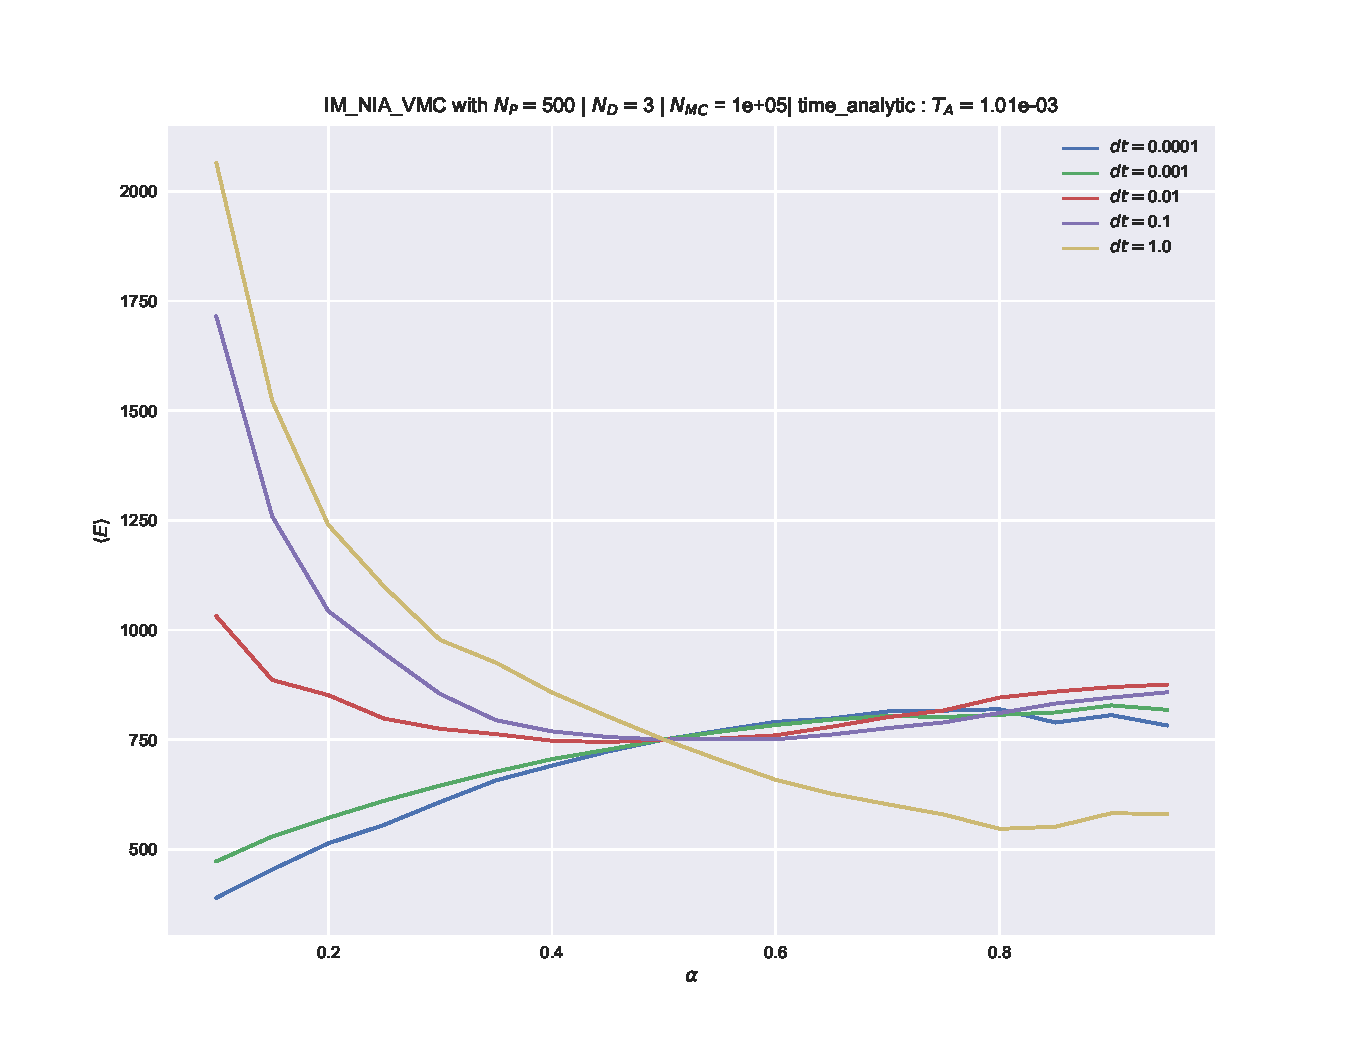
\includegraphics[width = \paperwidth]{figures/c_figs/IM_NIA_np_500_nd_3_dtcomparison.pdf}
\caption{Plot of simulations with 500 particles in 3 dimensions with varying timestep $dt$.}
\label{fig:1c_dt}
\end{figure}

\begin{figure}
\hspace{-2.8cm}
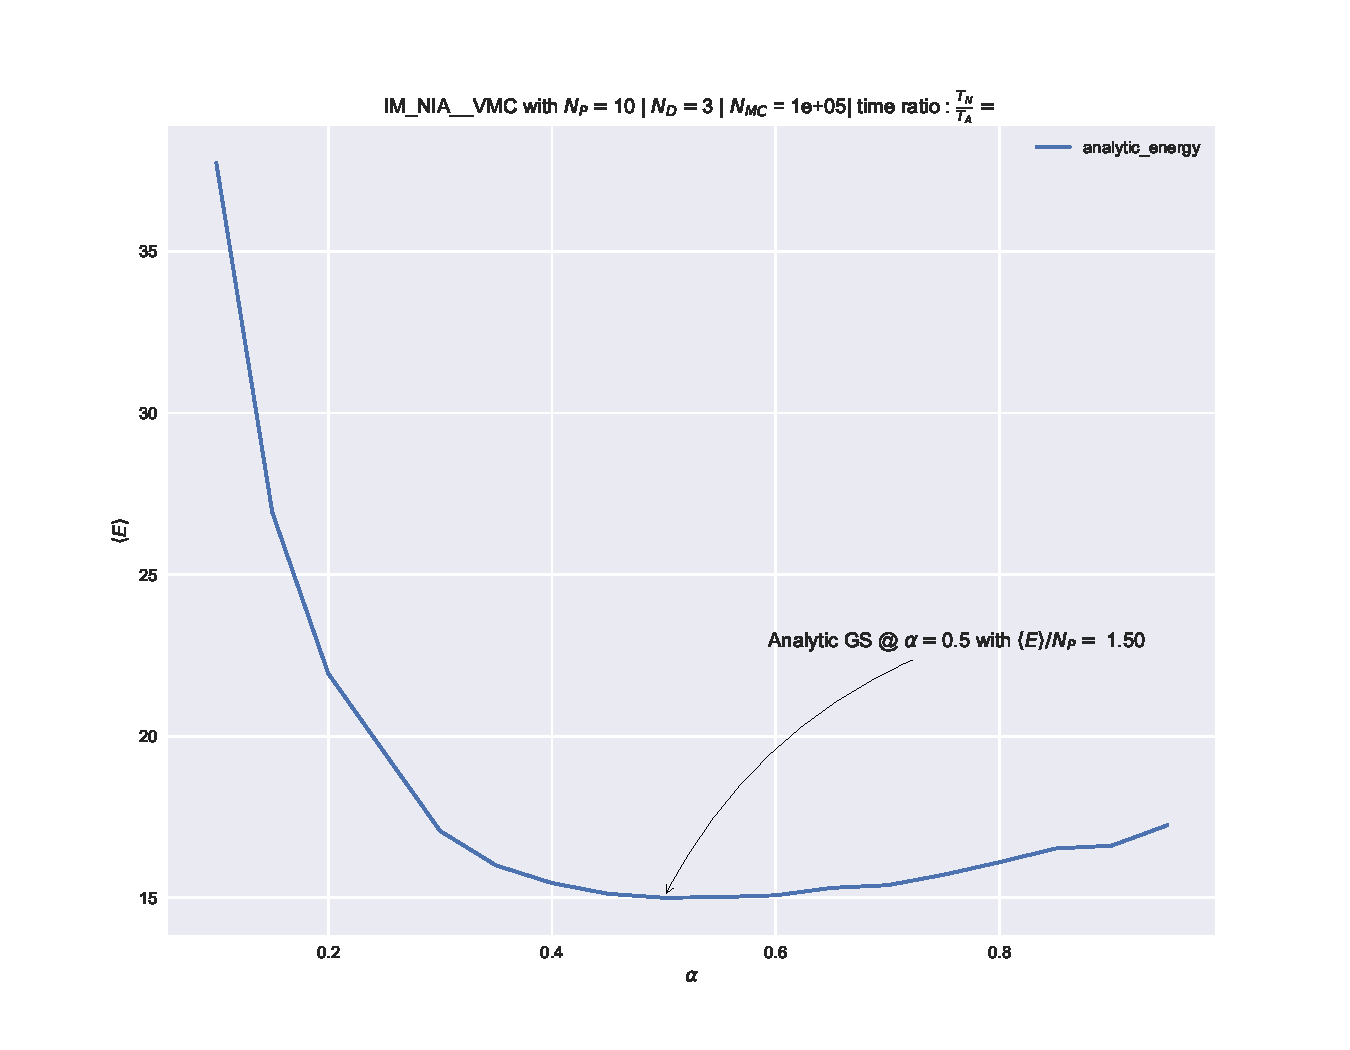
\includegraphics[width = \paperwidth]{figures/c_figs/IM_NIA_np_10_nd_3_dt_01_check.pdf}
\caption{Plot of simulations with 500 particles in 3 dimensions with varying timestep $dt$.}
\label{fig:1c_dt}
\end{figure}

\begin{figure}
\hspace{-2.8cm}
\begin{tabular}{cc}
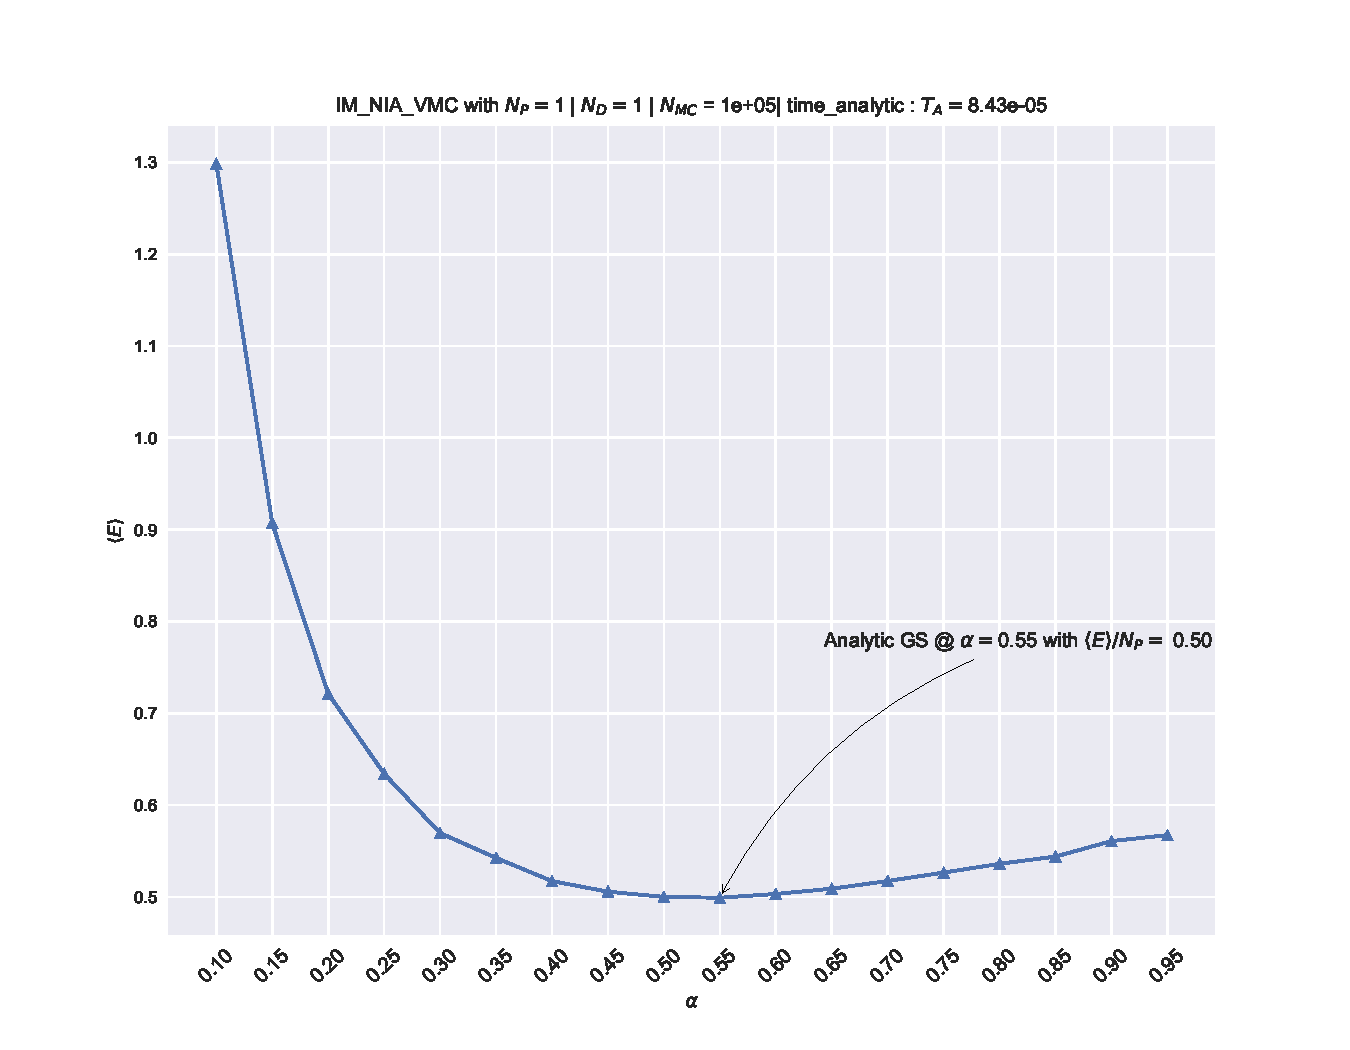
\includegraphics[width = 0.5\paperwidth]{figures/c_figs/IM_NIA_np_1_nd_1.pdf} & 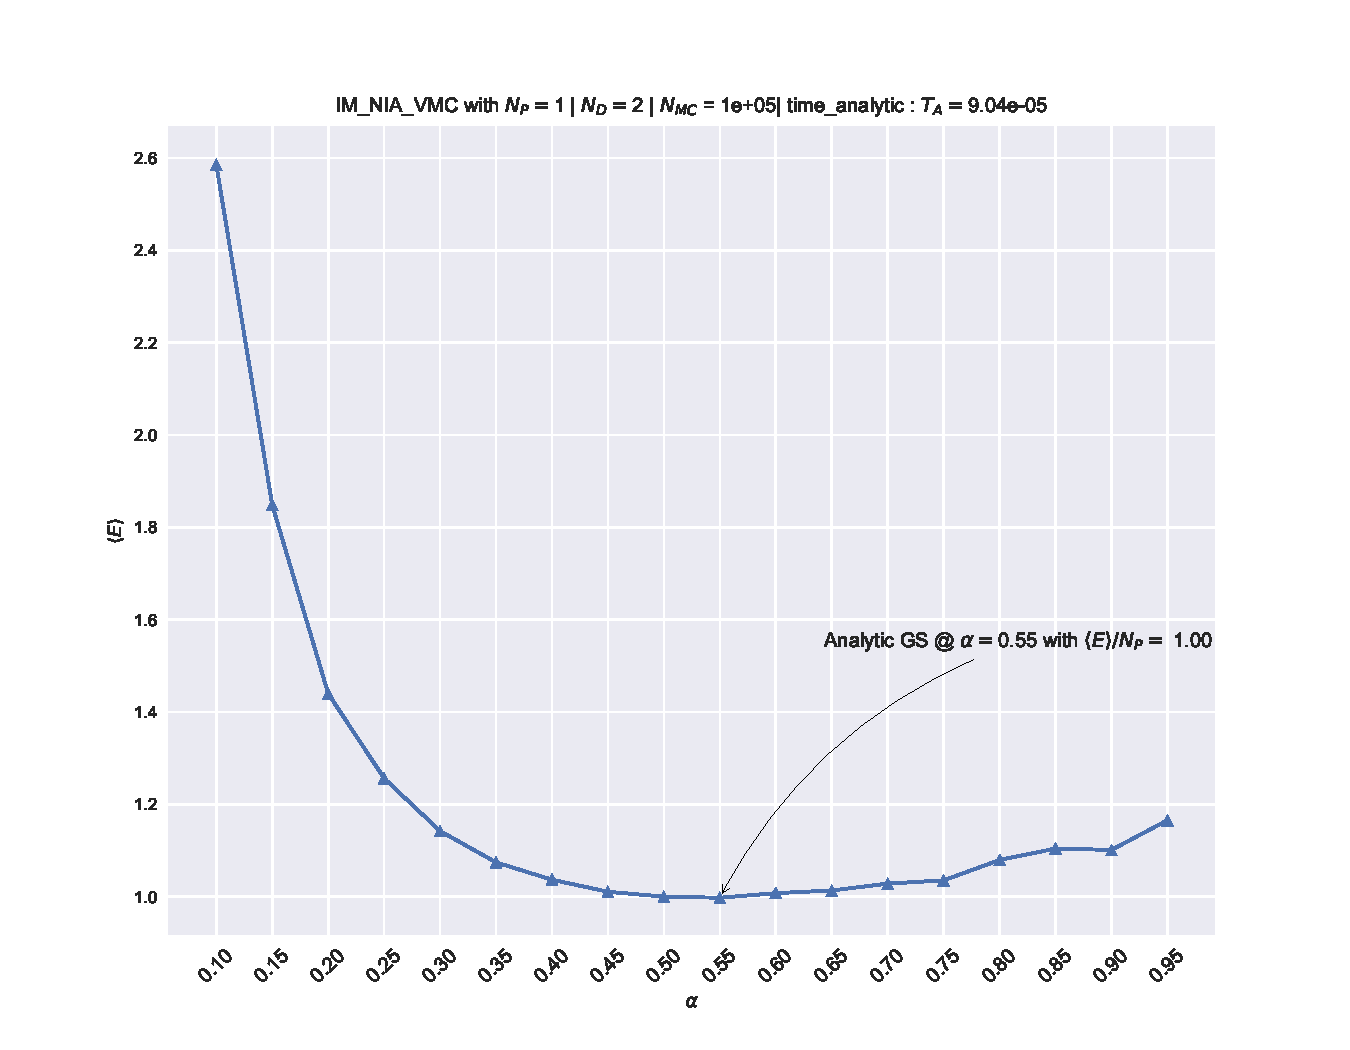
\includegraphics[width = 0.5\paperwidth]{figures/c_figs/IM_NIA_np_1_nd_2.pdf} \\
\multicolumn{2}{c}{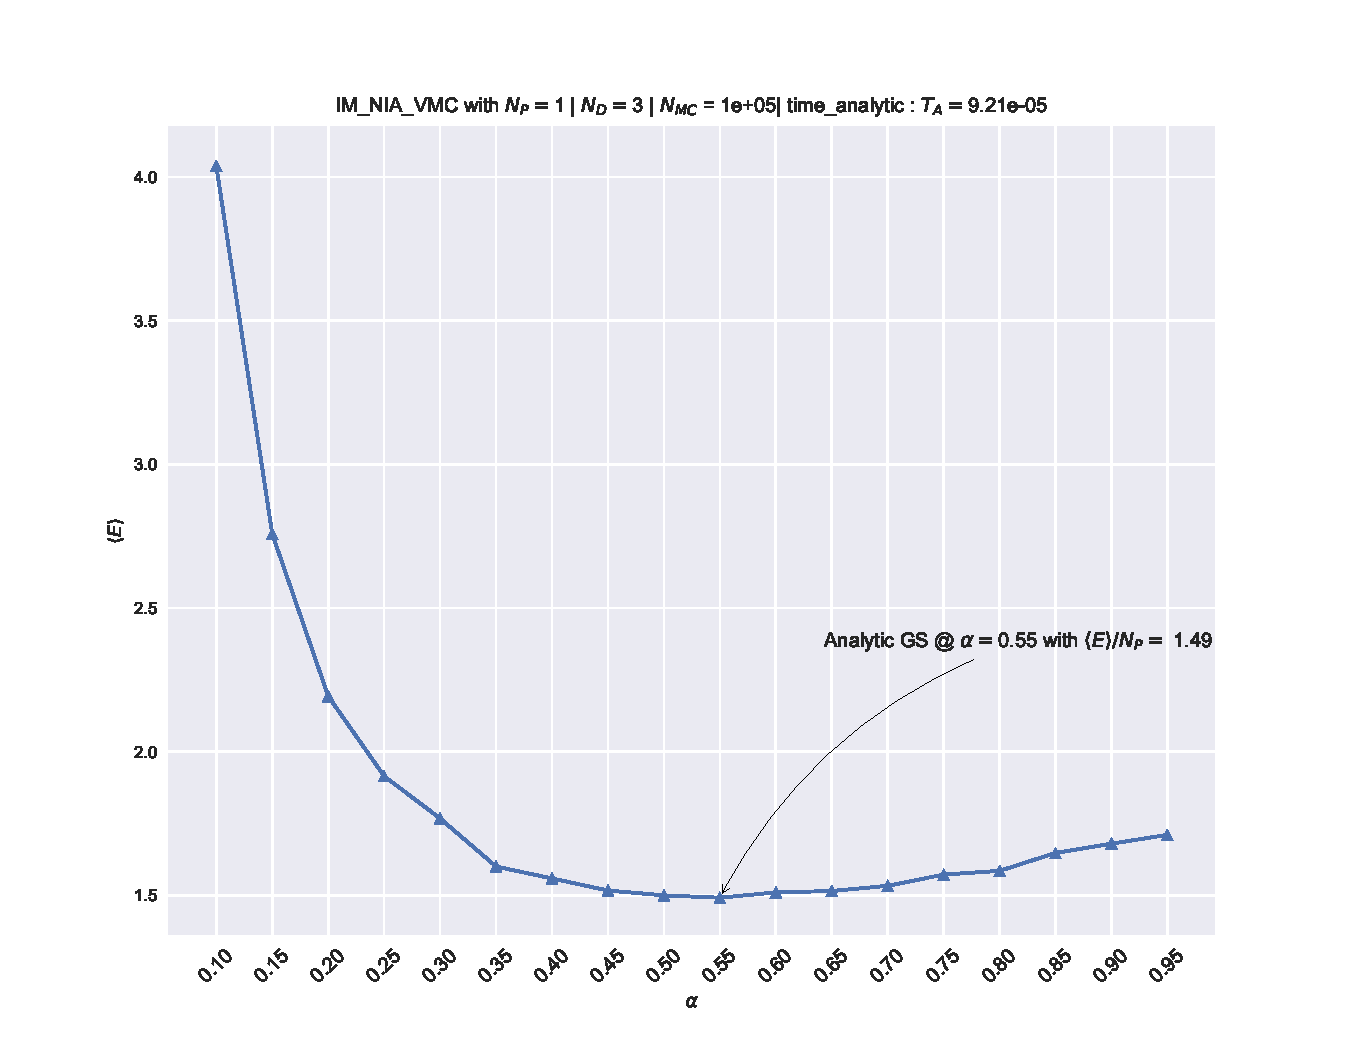
\includegraphics[width=0.5\paperwidth]{figures/c_figs/IM_NIA_np_1_nd_3.pdf} }
\end{tabular}
\caption{Plots for simulations with 1 particle and 1-3 dimensions.}
\label{fig:1c_1}
\end{figure}

\begin{figure}
\hspace{-2.8cm}
\begin{tabular}{cc}
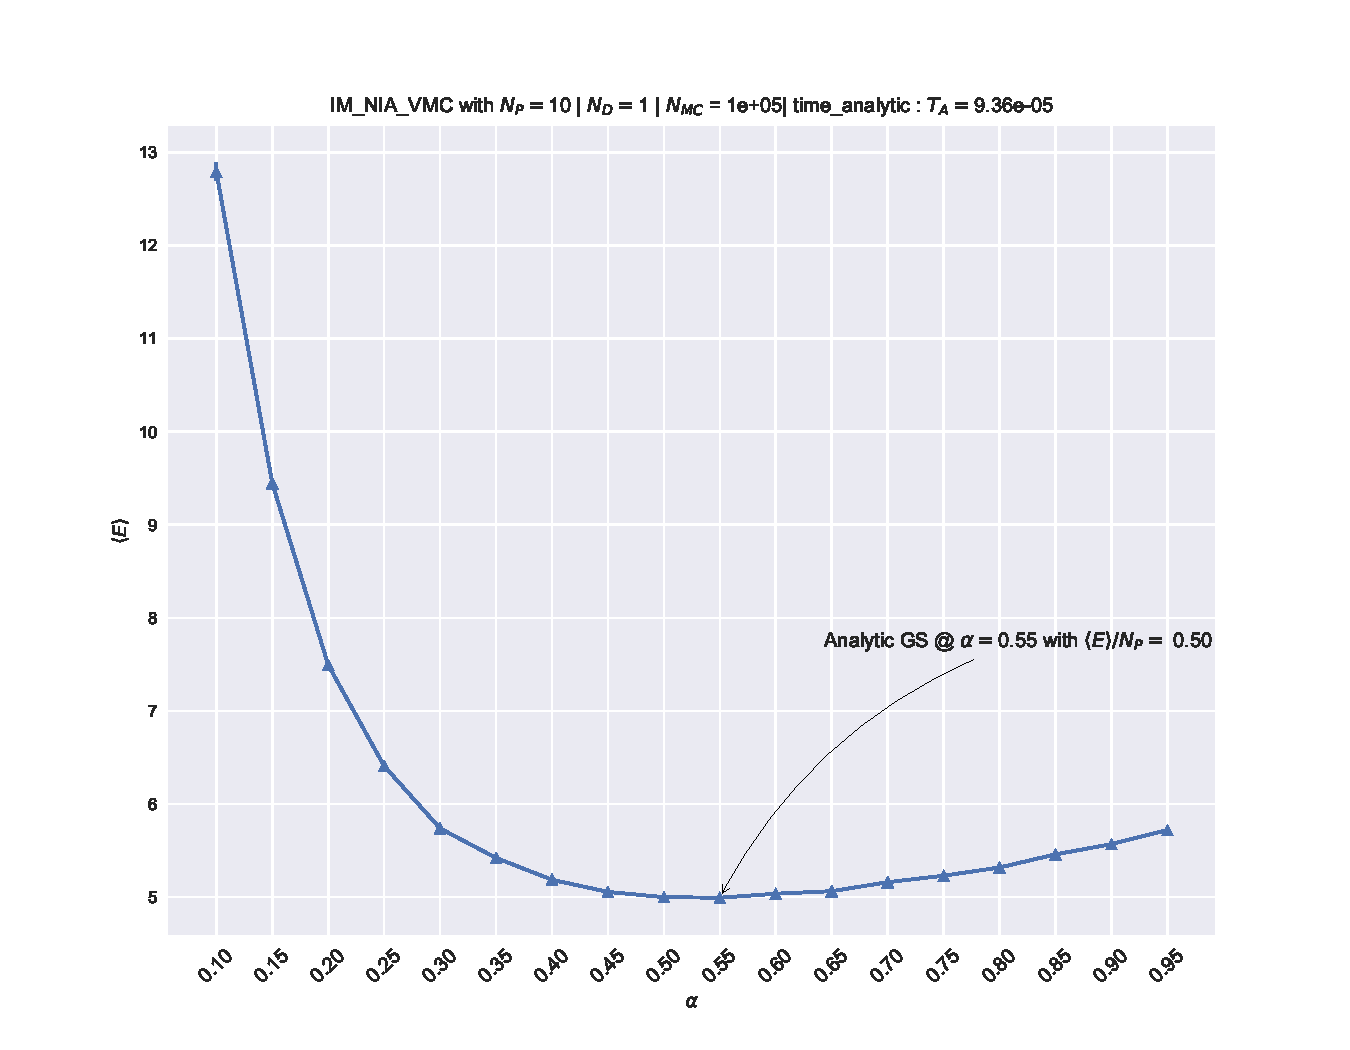
\includegraphics[width = 0.5\paperwidth]{figures/c_figs/IM_NIA_np_10_nd_1.pdf} & 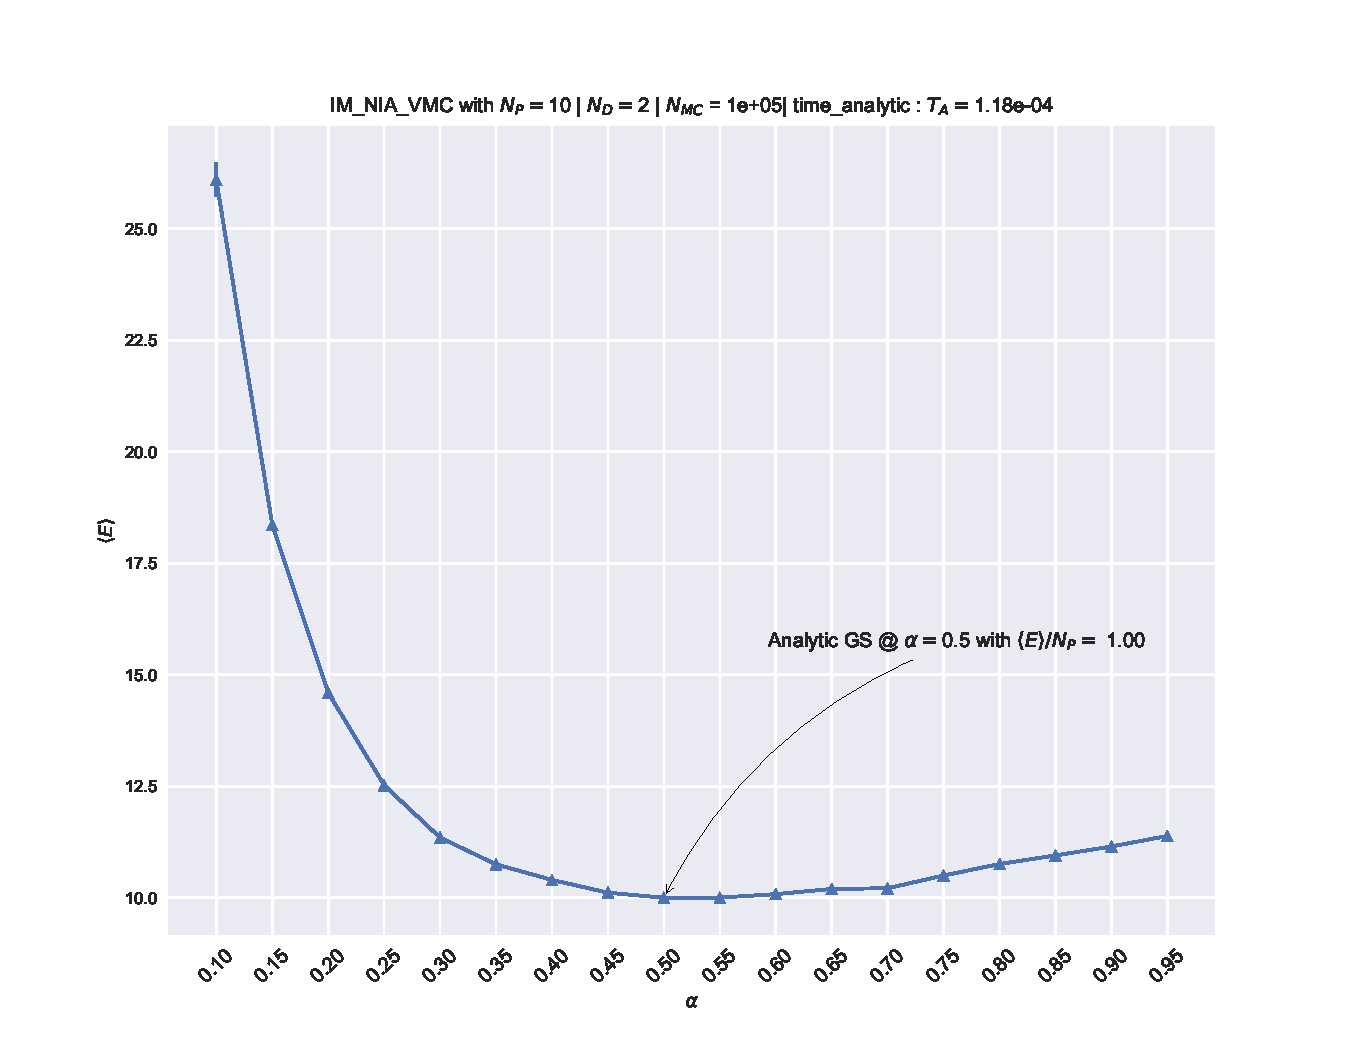
\includegraphics[width = 0.5\paperwidth]{figures/c_figs/IM_NIA_np_10_nd_2.pdf} \\
\multicolumn{2}{c}{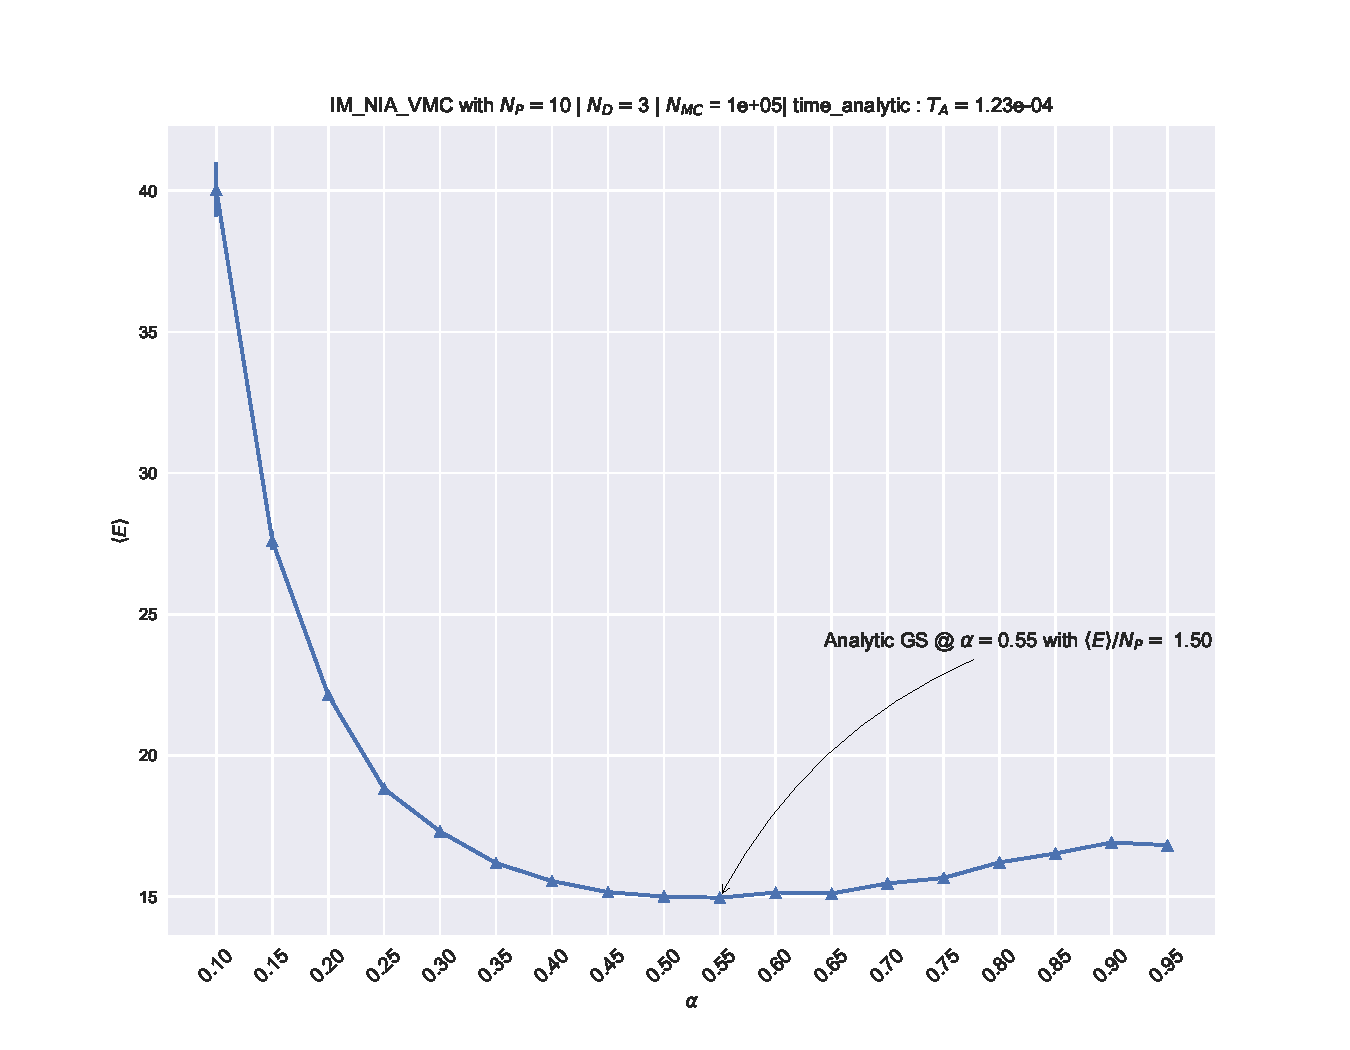
\includegraphics[width=0.5\paperwidth]{figures/c_figs/IM_NIA_np_10_nd_3.pdf} }
\end{tabular}
	\caption{Plots for simulations with 10 particles and 1-3 dimensions.}
\label{fig:1c_10}
\end{figure}

\begin{figure}
\hspace{-2.8cm}
\begin{tabular}{cc}
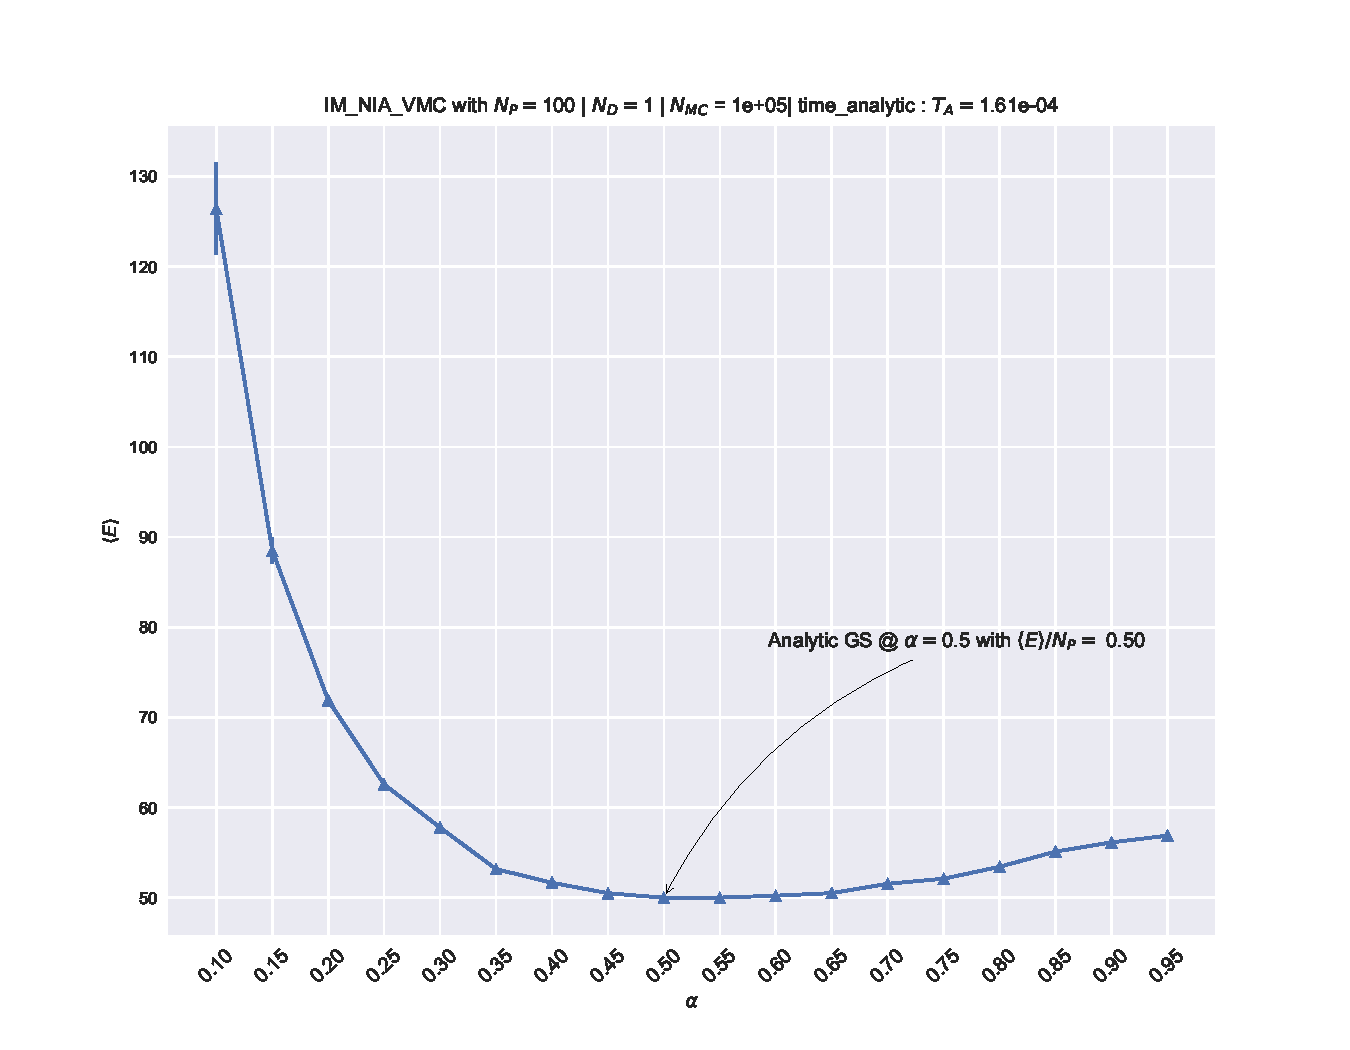
\includegraphics[width = 0.5\paperwidth]{figures/c_figs/IM_NIA_np_100_nd_1.pdf} & 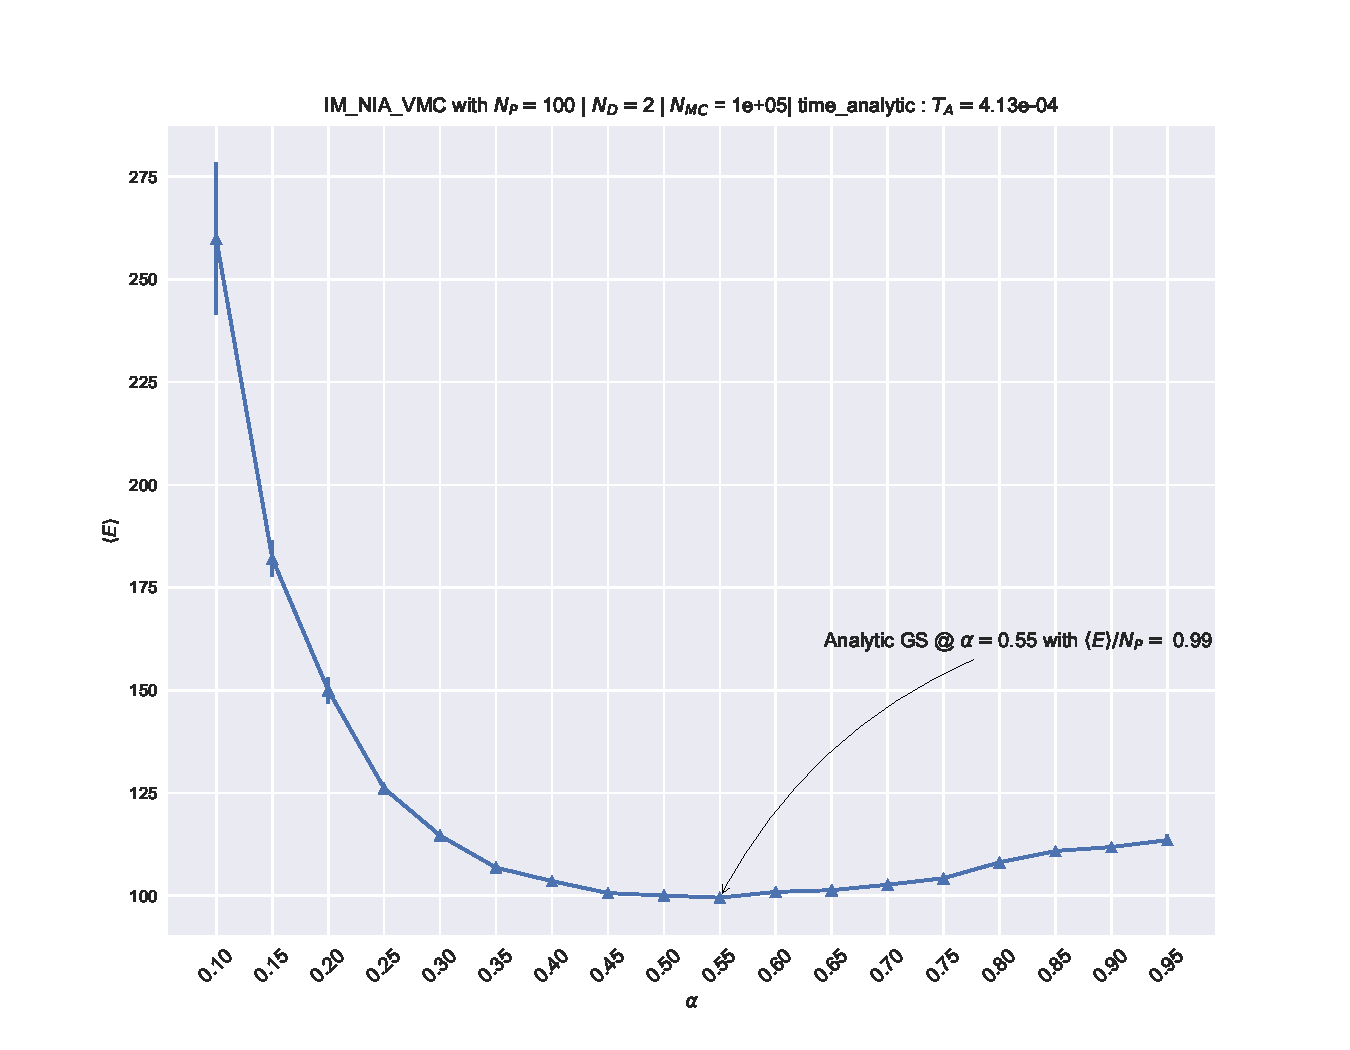
\includegraphics[width = 0.5\paperwidth]{figures/c_figs/IM_NIA_np_100_nd_2.pdf} \\
\multicolumn{2}{c}{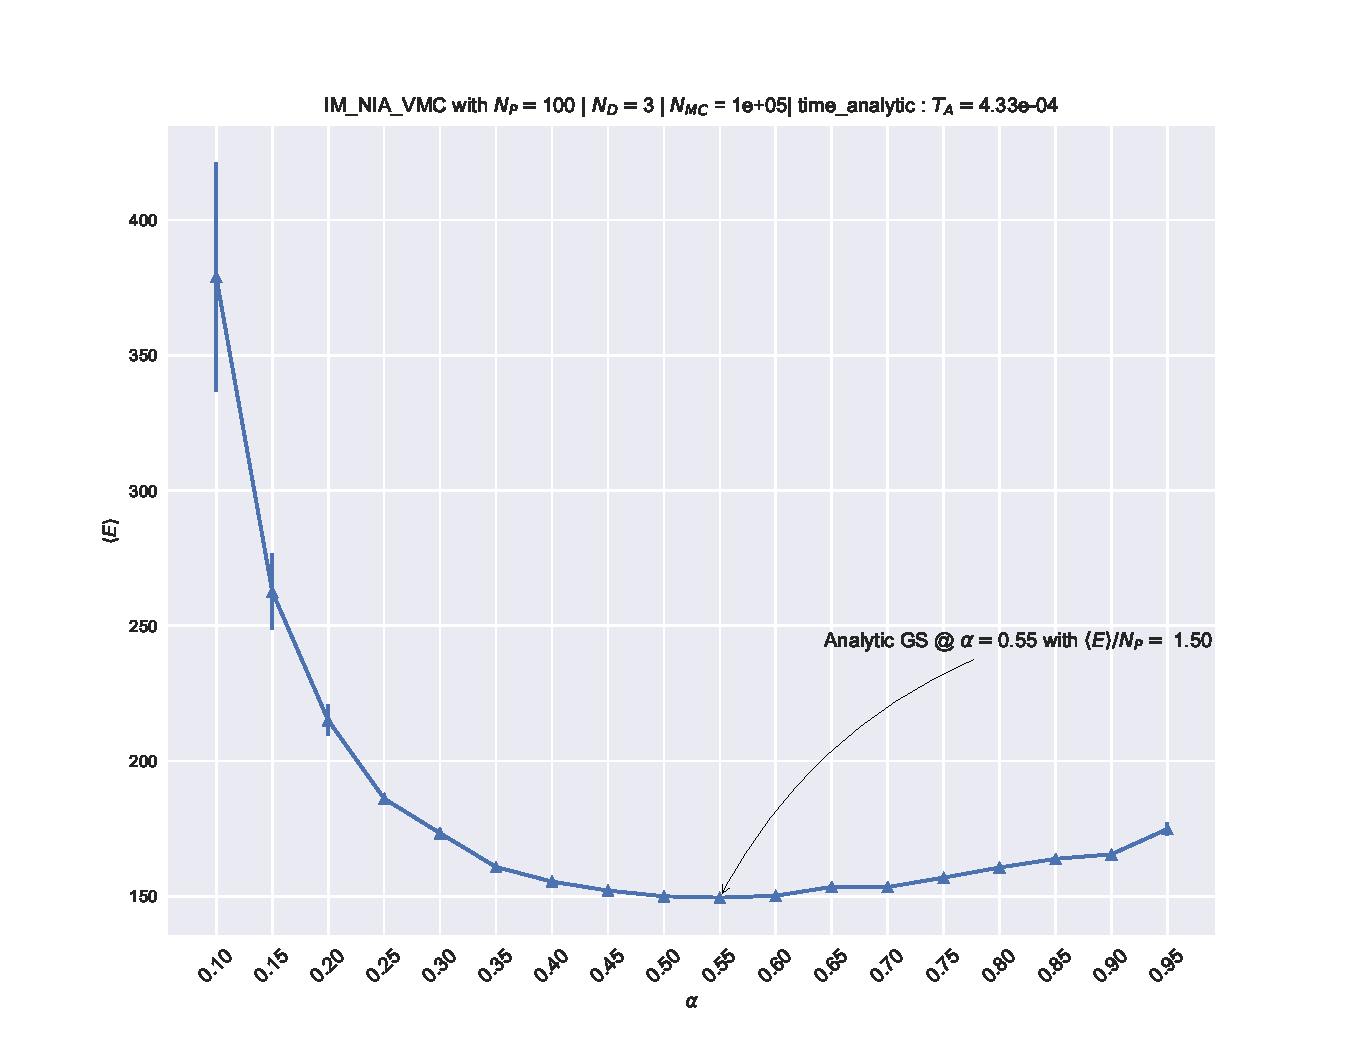
\includegraphics[width=0.5\paperwidth]{figures/c_figs/IM_NIA_np_100_nd_3.pdf} }
\end{tabular}
\caption{Plots for simulations with 100 particles and 1-3 dimensions.}
\label{fig:1c_100}
\end{figure}
\begin{figure}
\hspace{-2.8cm}
\begin{tabular}{cc}
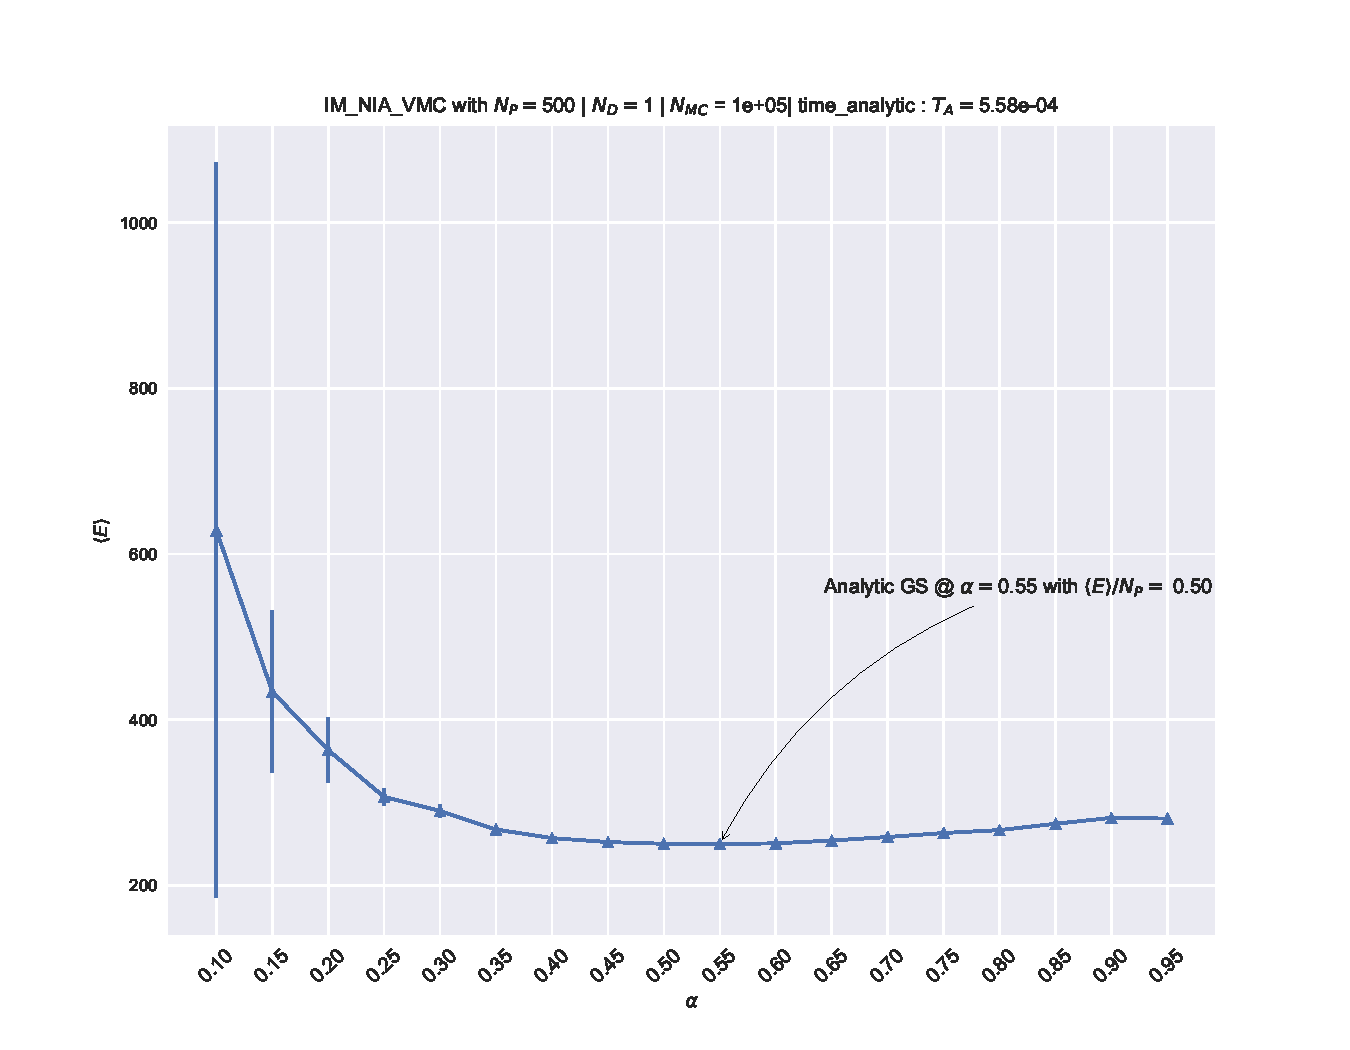
\includegraphics[width = 0.5\paperwidth]{figures/c_figs/IM_NIA_np_500_nd_1.pdf} & 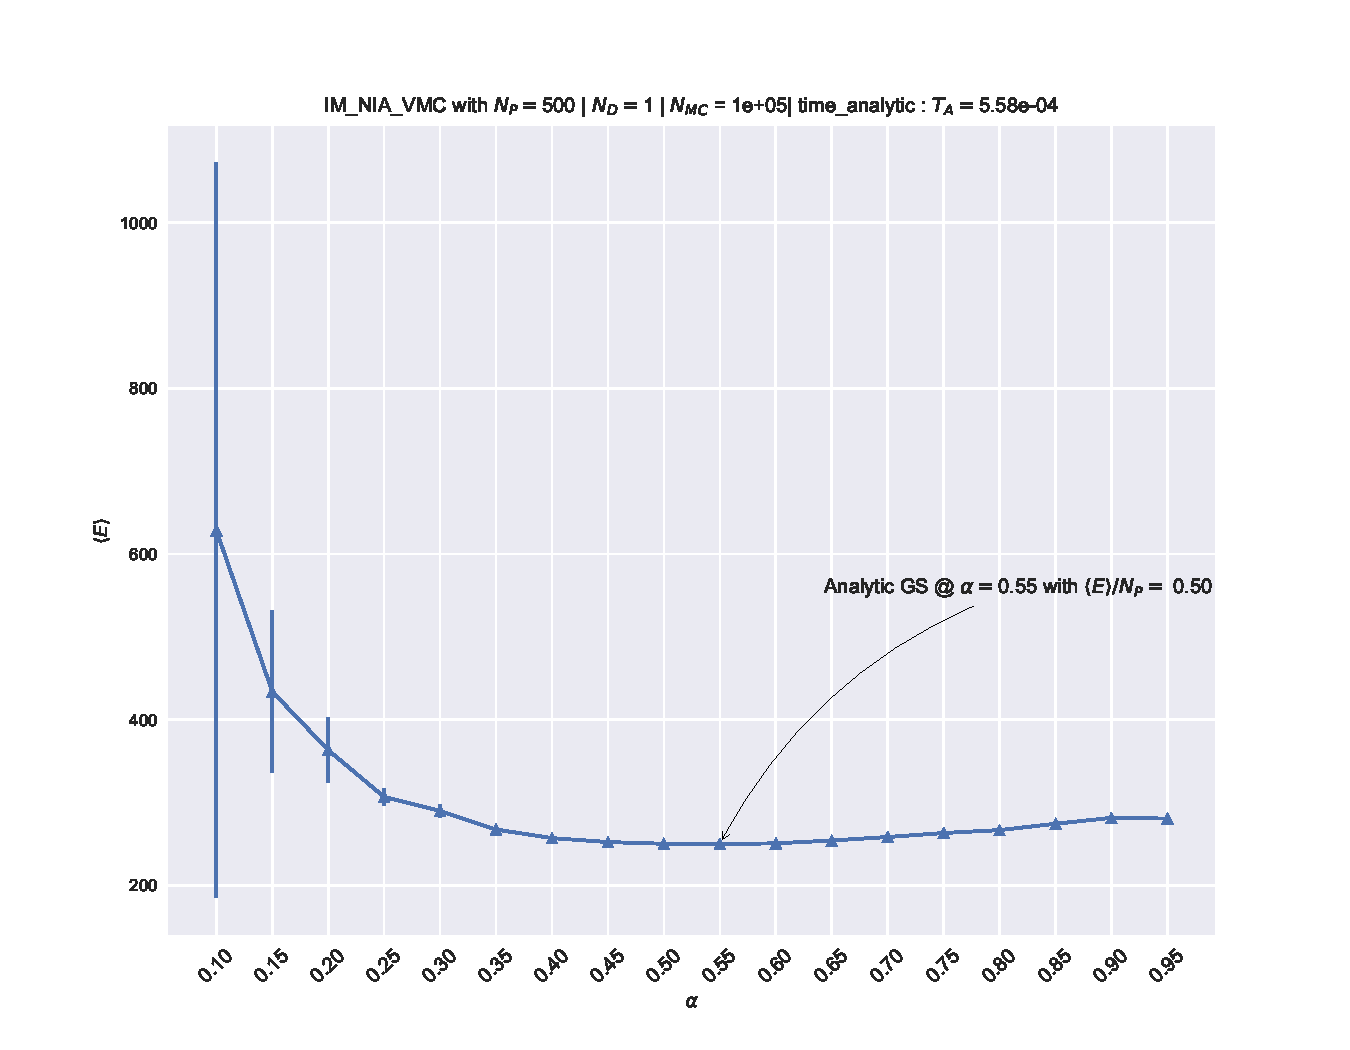
\includegraphics[width = 0.5\paperwidth]{figures/c_figs/IM_NIA_np_500_nd_1.pdf} \\
\multicolumn{2}{c}{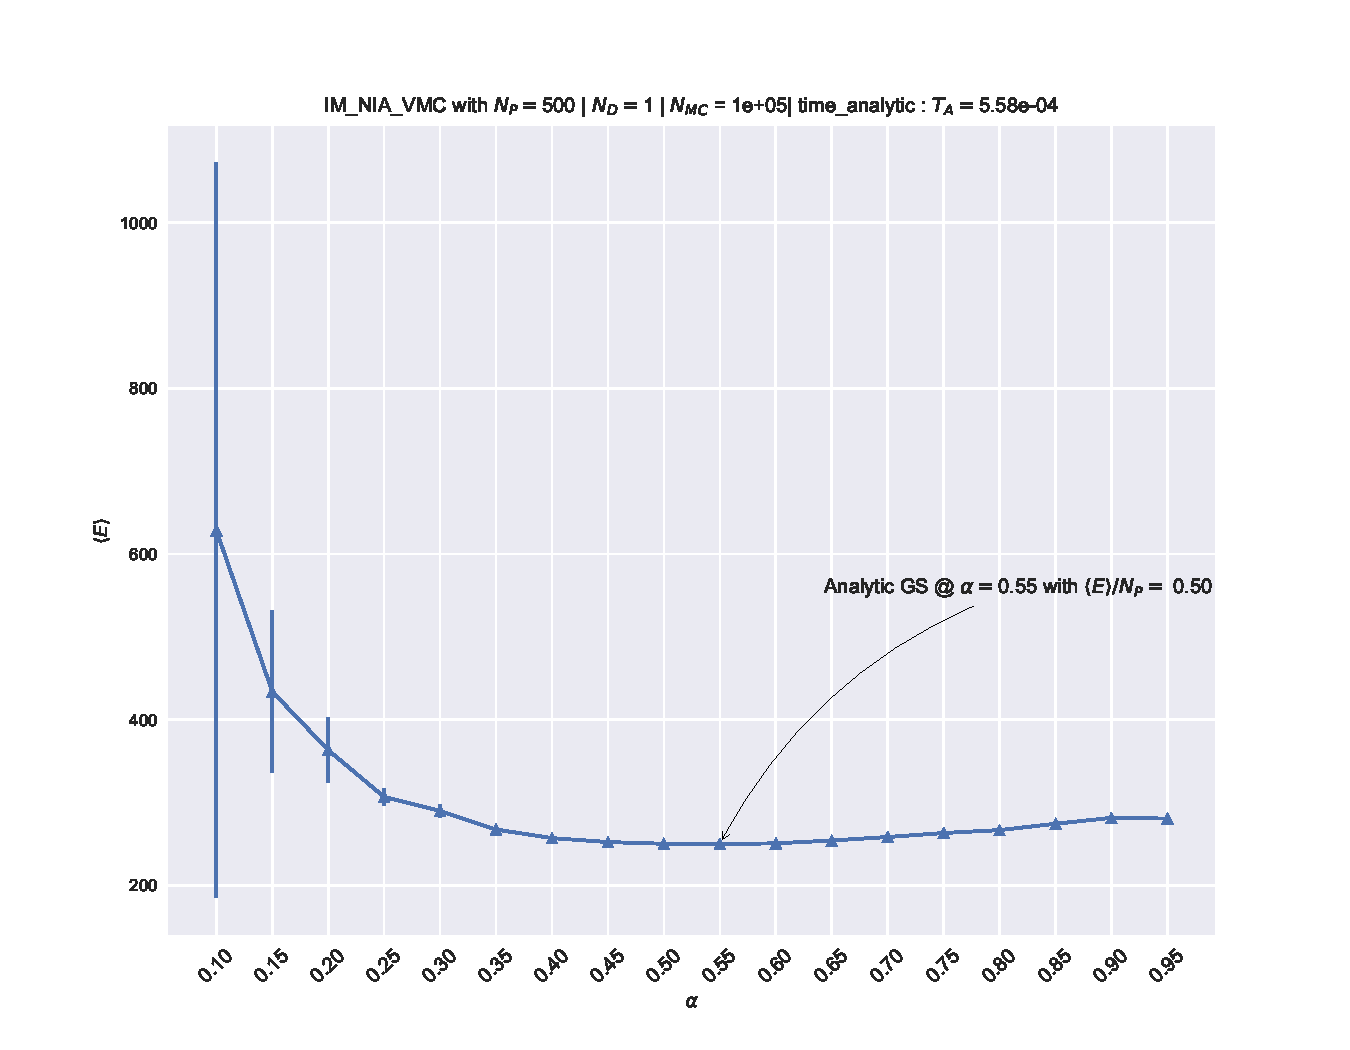
\includegraphics[width=0.5\paperwidth]{figures/c_figs/IM_NIA_np_500_nd_1.pdf} }
\end{tabular}
\caption{Plots for simulations with 500 particles and 1-3 dimensions.}
\label{fig:1c_500}
\end{figure}

\begin{figure}
\hspace{-2.8cm}
\begin{tabular}{cc}
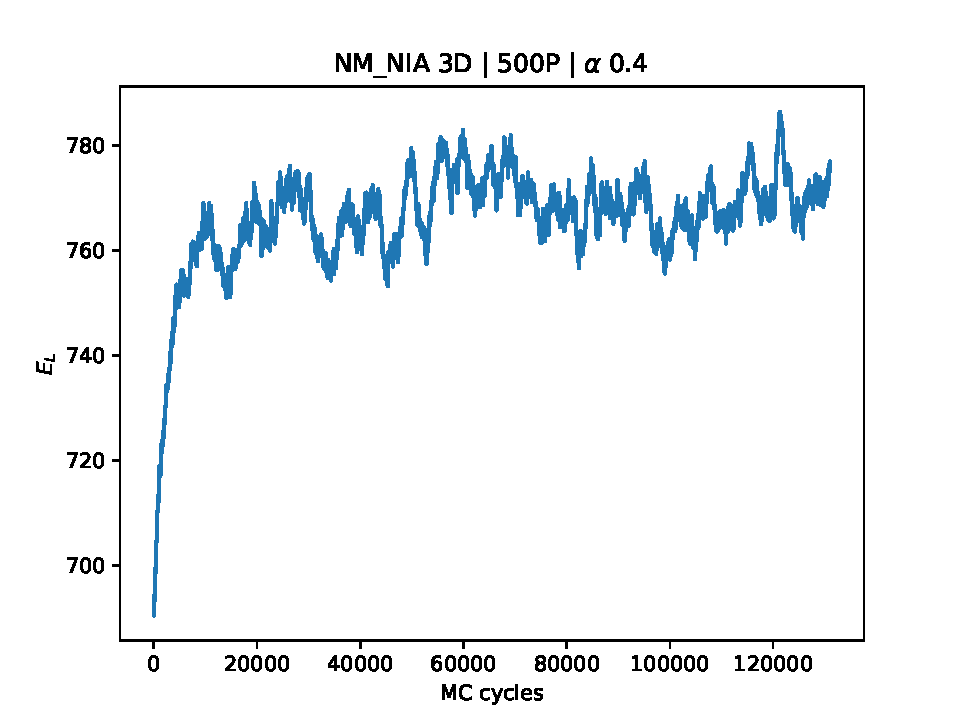
\includegraphics[width = 0.5\paperwidth]{figures/c_figs/NM_NIA_3D_500P_mc.pdf} & 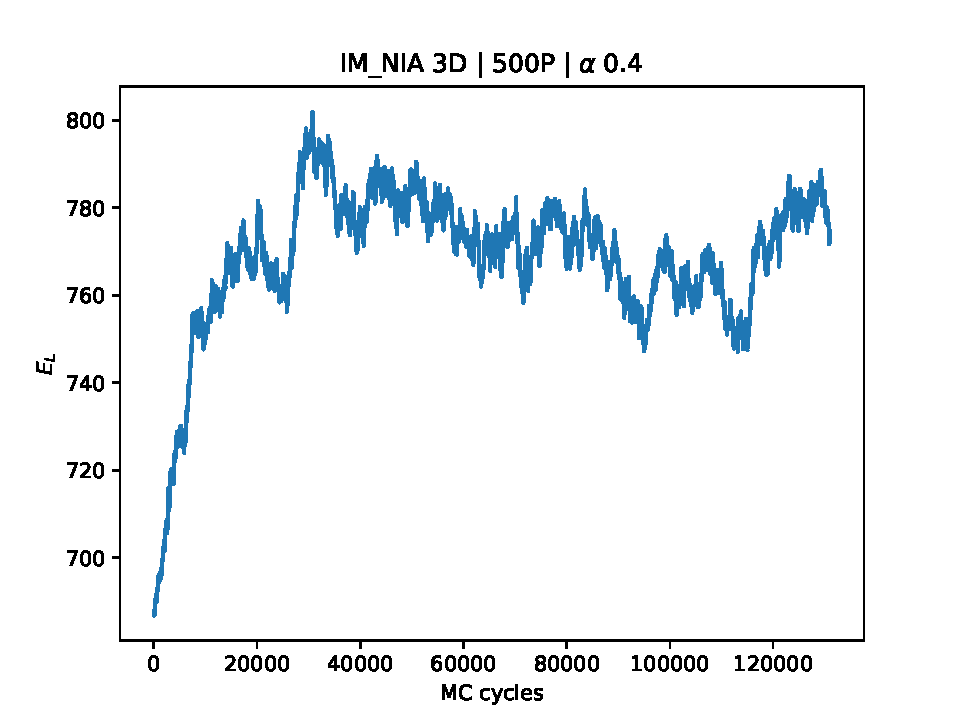
\includegraphics[width = 0.5\paperwidth]{figures/c_figs/IM_NIA_3D_500P_mc.pdf} \\
%\multicolumn{2}{c}{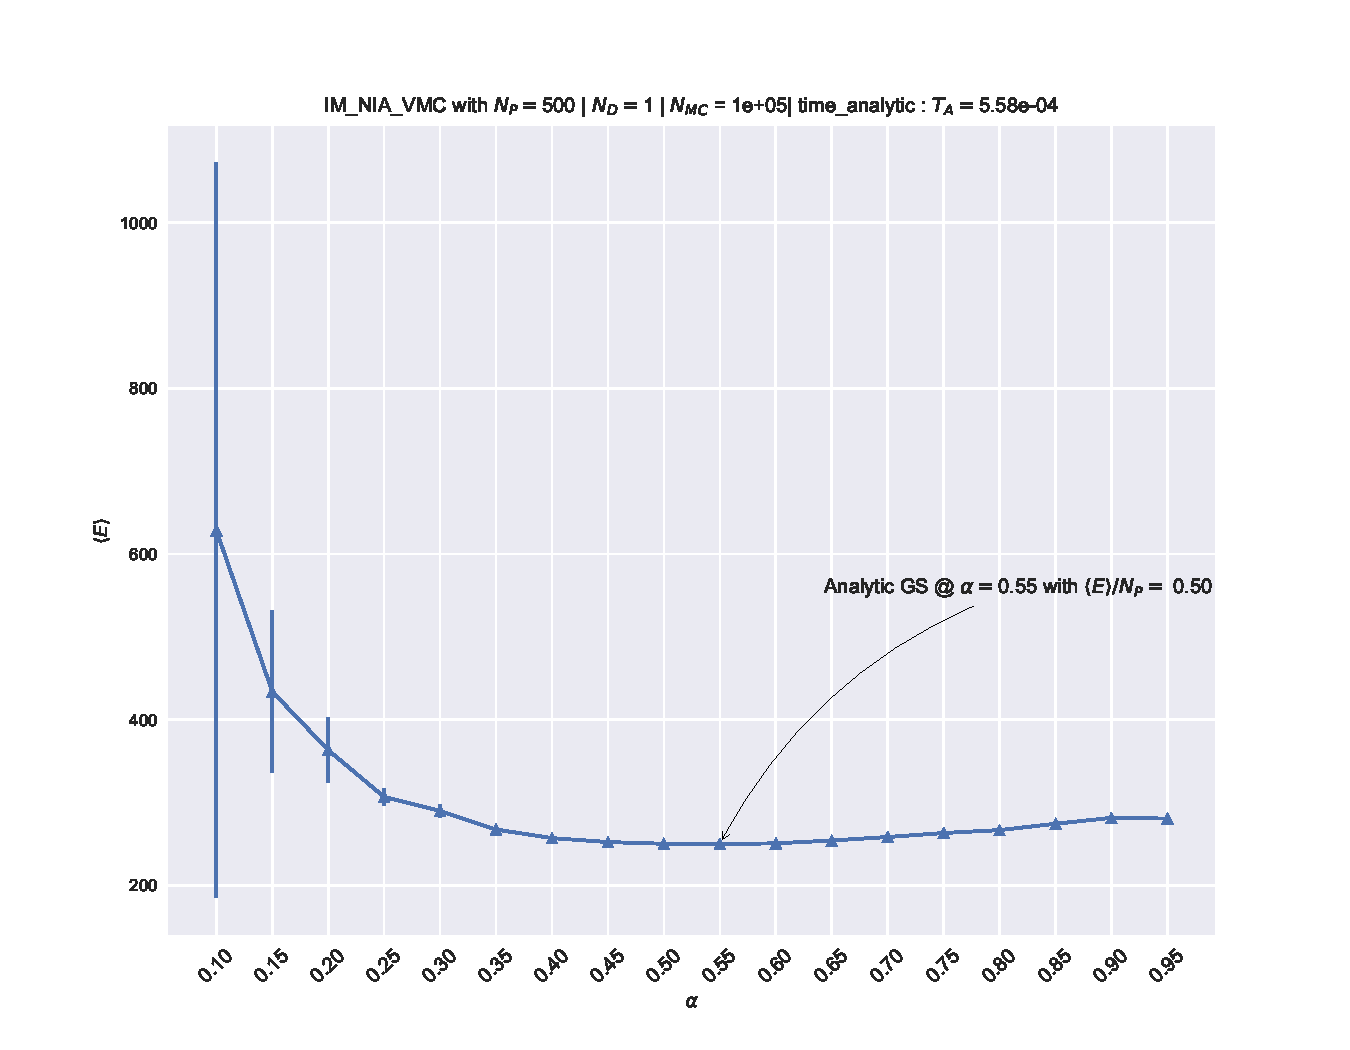
\includegraphics[width=0.5\paperwidth]{figures/c_figs/IM_NIA_np_500_nd_1.pdf} }
\end{tabular}
\caption{Plots for simulations with 500 particles in 3 dimensions showing the change in $E_L$ as a function of Monte-Carlo cycles.}
\label{fig:1c_mc}
\end{figure}
